\hypertarget{sec:2}{%
\section{Background, Prior Work, and Scope}\label{sec:2}}

\hypertarget{sec:2-1}{%
\subsection{Fingerprint Consistency and Contextual References}\label{sec:2-1}}

Fingerprinting research examines relationships as well as individual attributes. FP-Scanner detects countermeasure-induced inconsistencies, including discrepancies across JavaScript and HTTP reports \cite{ref04}. Picasso compares canvas challenge responses against device-class expectations \cite{ref05}. FP-Inconsistent studies spatial and temporal inconsistencies in evasive bot traffic \cite{ref06}. BrowserFM models dependencies among fingerprints, system characteristics, and browser configurations \cite{ref07}. Our study builds on this use of consistency as evidence.

WebView research examines both sides of the application--Web boundary. WVProfiler studies fingerprint exposure through Android WebView instrumentation \cite{ref08}; Tracking Without Borders examines tracking across Java/Kotlin, JavaScript, and runtime behavior \cite{ref09}; Cross-Boundary Mobile Tracking studies Java-to-JavaScript information diffusion \cite{ref10}. Our focus is a current Web report's compatibility with associated Android device and container measurements, including relation applicability, missing evidence, and behavior under edits and legitimate changes. Table~\ref{tab:related} maps these research scopes.

% Table 1 is registered early in Section 1 to keep the float on Section 2's page.

\hypertarget{sec:2-2}{%
\subsection{Observation Surfaces and Conditional Compatibility}\label{sec:2-2}}

Let \(E\) denote the execution state and container context. An observation \(x = (N(E), H(E), W(E))\) associates Native system and hardware measurements, WebView Host context, and App Web reports. The App schema has 177 catalogued fields: 84 Native, 26 Host, and 67 App Web. An optional Browser contributes 67 fields from a separate Web execution, yielding a 244-field paired schema when validly associated. Selected detectors use subsets of these fields. Association does not imply atomic sampling, and no surface is trusted ground truth.

\begin{figure*}[t]
  \centering
  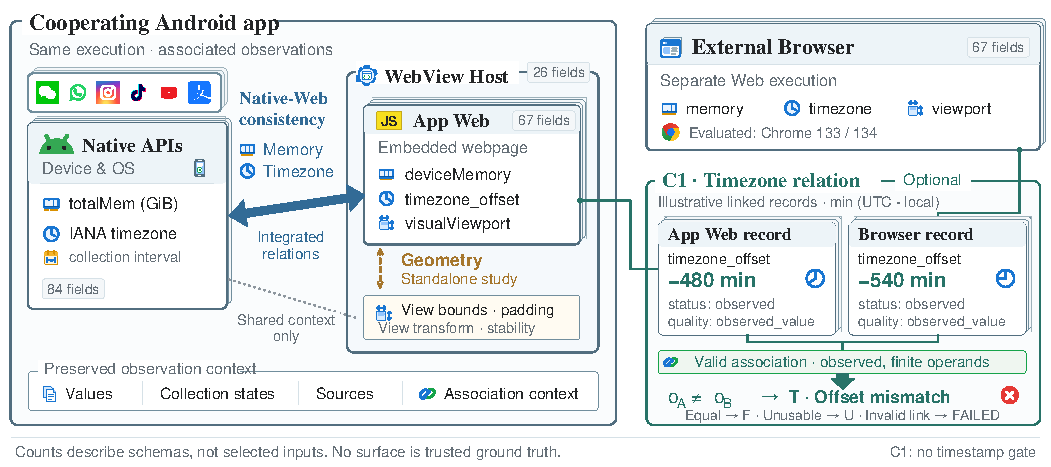
\includegraphics[width=\textwidth]{figures/HybridGuard_Fig1_surfaces_v4.pdf}
  \caption{Complementary observation surfaces in HybridGuard. Solid blue denotes integrated Native--App Web memory and timezone relations. Dashed ochre denotes the standalone Host--Web geometry study, outside Integrated App and its candidate pool. The dotted Native--Host edge represents shared context only. A validly linked external Browser supports the optional C1 timezone comparison with App Web. Counts describe catalogued schema fields, not the inputs of every selected detector.}
  \label{fig:surfaces}
  \Description{Native, WebView Host, and App Web observations form complementary surfaces. Memory and timezone relations are integrated; Host geometry is a separate study. An external Browser supplies an optional linked timezone reference.}
\end{figure*}


A semantic relation \(C_j\) constrains observations within a stated applicability domain. A local edit may replace \(W(E)\) with \(W^{\prime}(E)\) while leaving a reference unchanged; a legitimate change may move related observations together. Compatibility need not mean equality because APIs expose different units, precision, or abstractions. \(E\) is explanatory notation, not ground truth available to the detector.

We call a violation within an applicable relation \textbf{conditional report-integrity evidence}: the jointly observed values violate the declared constraint. This identifies an incompatibility without determining which operand was altered or establishing either operand's truth. A trigger counts as a detection only on a known effective modification.

\hypertarget{sec:2-3}{%
\subsection{Adversary and Claim Boundary}\label{sec:2-3}}

We use controlled browser overrides or emulation to edit resource, browser, locale, display, and graphics reports exposed to the Web application while a compared reference may remain unchanged. An operation counts as effective only when its effect is observed at the target surface. The detector receives the current observation, without operation labels, earlier baselines, or recovery records.

The intended setting is a cooperating Android application that collects Native and Host measurements alongside its embedded webpage. An ordinary remote website needs such integration to obtain these observations. Native and Host measurements are themselves mutable; being outside a local Web override does not make them administratively or statistically independent.

An alert supplies evidence of report incompatibility, not malicious intent, account takeover, or attacker identity. Conversely, no alert does not certify authenticity. An adversary may preserve the selected relations through either local or coordinated changes. We do not evaluate resistance to collector or backend compromise or adaptive evasion. Tracking and device re-identification are outside the evaluation.
